% !TEX TS-program = xelatex
\documentclass[11pt,a4paper]{report}

%---------------------------------------------------------------------------
% Packages
%---------------------------------------------------------------------------
\usepackage[margin=2.5cm]{geometry}
\usepackage{setspace}
\usepackage{lmodern}
\usepackage[T1]{fontenc}
\usepackage[utf8]{inputenc}
\usepackage{graphicx}
\graphicspath{{assets/}}
\usepackage{subcaption}
\usepackage{booktabs}
\usepackage{longtable}
\usepackage{float}
\usepackage{caption}
\usepackage{amsmath,amssymb}
\usepackage{hyperref}
\usepackage[numbers,sort&compress]{natbib}
\usepackage{tocloft}
\usepackage{fancyhdr}
\usepackage{listings}
\usepackage{xcolor}
\usepackage{natbib}
\usepackage{tikz}
\usetikzlibrary{shapes,arrows.meta,positioning,fit}
\captionsetup[table]{font=footnotesize, labelfont=footnotesize, justification=centering}
\captionsetup[figure]{font=footnotesize, labelfont=footnotesize, justification=centering}

%---------------------------------------------------------------------------
% Graphics and Listings Setup
%---------------------------------------------------------------------------
\captionsetup{font=small,labelfont=bf}
\lstset{
  basicstyle=\ttfamily\small,
  breaklines=true,
  frame=single,
  numbers=left,
  numberstyle=\tiny,
  keywordstyle=\color{blue},
  commentstyle=\color{gray},
  stringstyle=\color{teal},
  showstringspaces=false
}

%---------------------------------------------------------------------------
% Header and Footer
%---------------------------------------------------------------------------
\pagestyle{fancy}
\fancyhf{}
\fancyhead[LE,RO]{\thepage}
\fancyhead[RE]{\nouppercase{\leftmark}}
\fancyhead[LO]{\nouppercase{\rightmark}}
\renewcommand{\headrulewidth}{0.4pt}

%---------------------------------------------------------------------------
% Spacing
%---------------------------------------------------------------------------
\onehalfspacing

%---------------------------------------------------------------------------
% Document
%---------------------------------------------------------------------------
\begin{document}

%-------------------- Front Matter --------------------
\begin{titlepage}
	\centering
	{\Huge\bfseries Title of the Thesis\\[1em]}
	{\Large Subtitle if needed\\[4em]}
	{\Large Jack Jibb\\[2em]}
	{\large School of Computing and Mathematical Sciences, University at Greenwich\\[1em]}
	{\large 2024-2025\\[4em]}
\end{titlepage}

% Abstract
\begin{abstract}
	% Add Abstract to ToC
	\addcontentsline{toc}{chapter}{Abstract}
	In professional cycling, athletes are often sent to training camps in locations such as the French Alps, Andorra, Sierra Nevada,
	Colorado Springs, or other high altitude destinations. While a big part of this is altitude acclimatisation, many cyclists report
	that the biggest effect is actually the suitability of the roads for training. Long, car-devoid mountains, where athletes can just
	put their head down and focus on their effort means that their training quality is improved, as opposed to having to ride through small
	villages, stopping at intersections and being constantly vigilant of overtaking cars or traffic furniture. This thesis explores the
	possibility of being able to track and quantize "Training Suitability" of roads. What is proposed is an integrated framework that
	can semantically partition continuous trajectory data from a cyclist's GPS device, and meaningfully define each segment in the context of
	training suitability. Starting from raw GPS traces, we apply geometric filtering and map-matching to correct noise and align positions with a
	reference network. An adaptive segmentation algorithm then identifies breakpoints using curvature statistics, speed variance,
	and road metadata (such as road name, or speed limit), yielding segments that have a homogenous quality.
	Each segment is characterized by spatial, temporal, and contextual features and subsequently classified through a Wavelet Transform
	function that quantizes variability and changepoints in data streams. The scalability and robustness of the framework will be evaluated
	through a small-scale live web application.

\end{abstract}

% Table of Contents, List of Figures, List of Tables
\tableofcontents
\listoffigures
\listoftables

%-------------------- Main Chapters --------------------

\chapter{Introduction}
\label{chap:introduction}
Modern cycling training for professional athletes has been perfected down to a science. Since the days of Team Sky, "marginal gains" and hyper optimisation
in all aspects of training, such as nutrition, periodization, strength, endurance and race calendar have been optimised to such a degree that
the difference between the top echelon of professional cycling and the middle tier is less than a few percent. Pro riders have the advantage of
having everything done for them when it comes to planning training, from their schedule to their locations. However, amateur riders do not have this
same advantage, and as I have experienced many times, often we go out for rides, looking for new, longer routes to do training on, only to find
that we end up down a country lane with blind corners, or a town with really annoying road furniture. The first step in planning a route has always
been to go onto a mapping website, and draw a route, that you could later save to your GPS device to follow, or to write down turn by turn on the stem of your
handlebar. While I won't mess with the sacred art of taping a piece of paper on your handlebars in the most aerodynamic way you can, I can maybe
just revolutionise the plotting of routes for cyclists looking to get the most out of their training. Enter the concept of route "segments". In Strava,
a Segment is a piece of road that has been given a place in their database, for athletes to compete for times on. Getting a "KOM" (King of the Mountain) on
a Strava segment is a coveted title by many amateurs. In our context, a segment will be keeping track of more than just performance metrics. It will
keep track of the inherent data of the road from an open source mapping software called OpenStreetMap, and all the data will be combined to give
an overall "score" of the segement in the context of training suitability.
\section{Background}


\section{Research Objectives}
\begin{enumerate}
	\item To develop a system that can take user cycling data in the form of GPX files, and provide feedback in the context of training suitability
	\item To design and implement a Route Segmentation algorithm that splits a GPX file into meaningful sections by enriching a route-matched
	      path from the data with road information from OpenStreetMap.
	\item To be able to store the segments in a database, and future GPX files can be converted into arrays of these segments, by matching their
	      segments with the database, and returning segments if there is a margin of error less than a certain threshold.
	\item To implement batch processing of GPX files so users can submit large quantities of GPX data to aid in segment generation.
	\item To create a two-way pipeline system that takes either GPX data, or a custom-plotted route, and feeds back a list of curated segments from the database.
\end{enumerate}





\chapter{Literature Review}
\label{chap:litreview}

\section{Training Suitability and Segmentation Algorithm Design and Analysis}

\subsection{Research Objectives}
\subsection{Algorithmic Approaches to Segmentation and Categorization}
\subsection{Applications in Cyclist Route Planning}
\subsection{Methodological Considerations and Assumptions}

\section{Training Suitability Scoring}

\subsection{Research Objectives}
\subsection{Approaches to Suitability Scoring}
\paragraph{Sharifzadeh et al. "Change Detection in Time Series Data Using Wavelet Footprints"}
An interesting approach to Suitability scoring relates to Fast Fourier Transforms, and a convolution approach comes from Medhi Sharifzadeh et al, from the University of Southern California, introducing a concept known as
"wavelet footprints" as a compact, multi-resolution approach to representation of spatial-temporal trajectories. Wavelet footprints are a  more granular version of the Wavelet Transform, which in turn is a version of the Fourier Transform. The approach involves using Wavelets to transform a signal into the "Wavelet Domain".
The smaller the wavelet, the more reactive it will be to change in the original signal, so by adjusting the size of the wavelet, the signal can be filtered to be more or less reactive to change.
Wavelet footprints have an advantage over the general Wavelet transform, where they only retain the most significant components. This is done by having wavelets occur in orthoganal sets.
Due to Heisenberg's Uncertainty Principle, it is impossible to perfectly describe both the frequency content of a signal and the location in time of the signal. Time-domain and Frequency-Domain analysis in this regard are
at opposite ends of the spectrum, but the Wavelet Domain sits in the middle, allowing for a sliding scale value, where a larger scale gives more frequency and less time resolution, while smaller scales give less frequency, and more time resolution.

The advantage of using wavelet footprints over the Fourier Transform means that it is possible to isolate points in the signal where significant changes occur in specific metrics, or combination of metrics, allowing flexibility in choosing
what conditions must be met to enact a segmentation.

\paragraph{Indoor Cycling Association: "How Much Time in the Red Zone?"}
This article details a breakdown of the 7-training-zone model, which provide a good template for cutoff times for tuning Wavelet Footprints for analysing the GPX signal.
The general consensus is having 5 zones is a good compromise between continuous training definitions (specific power numbers) and binary (hard or easy). While the article describes 7 zones,
Zones 1-3 all fall outside of the hour range, which for the purpose of segment analysis would be fairly useless. The 5-Zone model approach
has good suitability to wavelet analysis, since small scale values for a wavelet would detect short burst efforts, while larger scales will detect longer, sustained effort.
Having 5 zones allows for a reduced scale array, contributing to higher performance. Here is a graphic, courtesy of the Indoor Cycling Association, that breaks down each zone. Zones 3-7 will be used for Wavelet Analysis.
\begin{figure}[h!]
	\begin{center}
		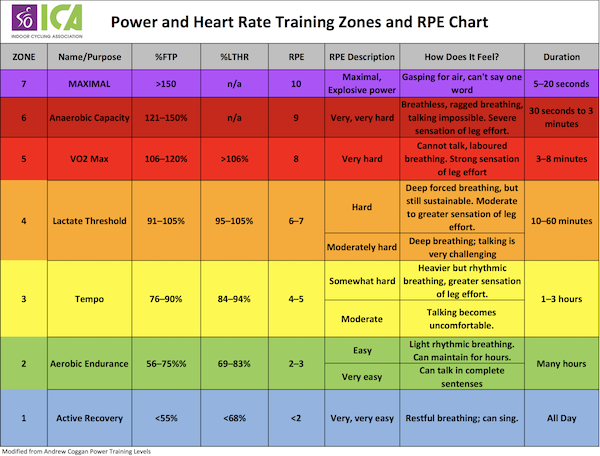
\includegraphics[width=0.6\textwidth]{zones.png}
	\end{center}
	\caption{The 7 Zone Training Model, courtesy of Indoor Cycling Association}
\end{figure}

\paragraph{Sean Hurley: "Normalized Power: What It Is and How to Use It" https://www.trainerroad.com/blog/normalized-power-what-it-is-and-how-to-use-it/}
TrainerRoad writer Sean Hurley provides a useful and consise definition of Normalized Power (NP), a metric invented by Dr. Andrew Coggan in his book \textit{Training and Racing With a Power Meter}. NP
"reflects the disproportionate metabolic cost of riding at high intensity, by weighting hard efforts and deemphasizing periods of easy spinning", according to Dr Coggan.
Essentially, NP approximates what power a rider could have put out for the same effort, if their effort was steady-state. While it is not a completely accurate metric for effort, it is a really
good indication of power variability, and as such is useful in determining the type of effort of a segment. The algorithm for determining NP is as follows:
\begin{enumerate}
	\item Calculate a rolling 30 second average power for the duration
	\item Raise each rolling average value to the fourth power.
	\item Determine the average of all the rolling values
	\item Take the fourth root.
\end{enumerate}
For an input power signal, $P(t)$ over interval $(0,N)$, the formula for Normalized Power (NP) is:
\[
	\mathrm{NP} = \bigg( \frac{1}{N} \sum_{i=1}^{N}\big(\overline{P}_{r}(i)\big)^{4}\bigg)^{1/4}
\]
where $P_r$ is the 30 second rolling average power starting at point i in the power data array.
\subsection{Applications in Training Suitability Scoring}
\subsection{Methodological Considerations and Assumptions}
\begin{itemize}
	\item \textbf{Power:} All cyclists have different power thresholds; in other words, two cyclists may be going the same speed up a climb, but one may be going all out, and another just going easy.
	      They may not even have the same power output. The one going easy could have a higher power output than the person going all out, depending on their weight. As such absolute power is a bad reference
	      point for training suitibility. Rather, we need to focus on power variation, as well as power curve. A power curve is the integration of all power numbers over a duration of exercise, plotted average power in watts on the y-axis,
	      and max sustained duration for that average power on the x-axis. The graph tends to look like an exponential decay function. An example of my own personal cumulative power curve in 2024 is shown here:
	      \begin{figure}[h!]
		      \centering
		      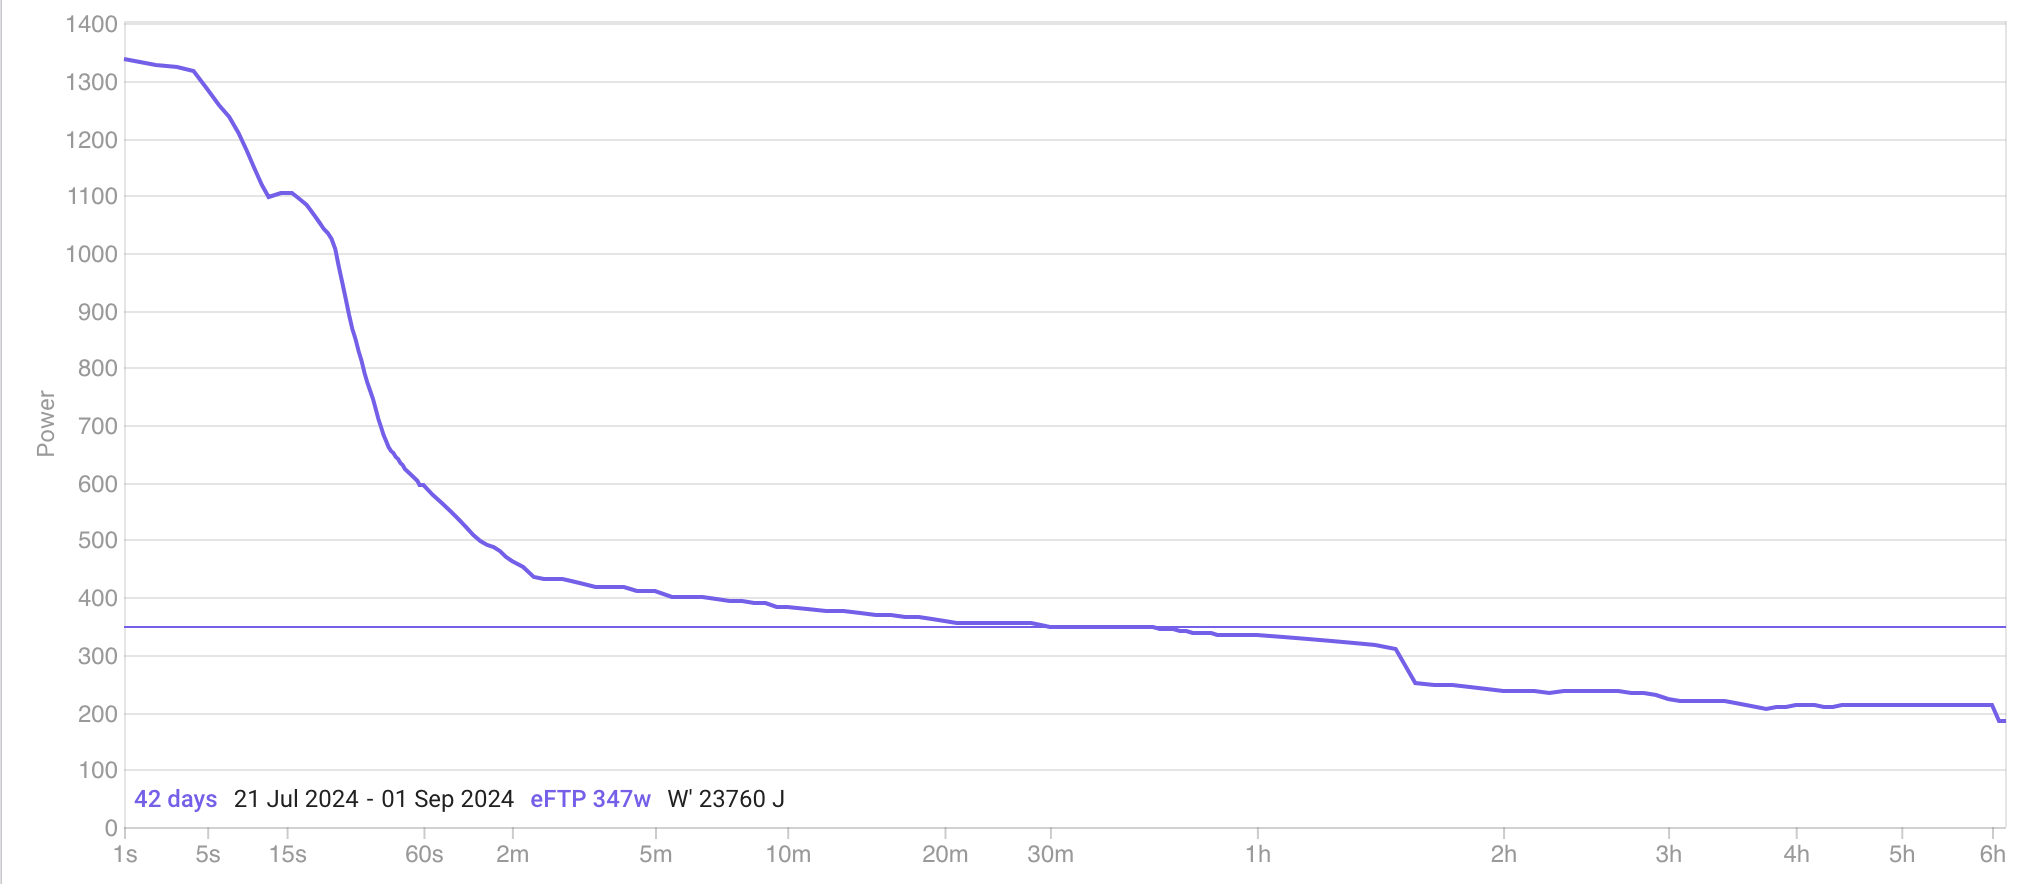
\includegraphics[width=0.8\textwidth]{jibb_powercurve.png}
		      \caption{My Power Curve for August, 2024. The power curve can estimate what would be considered "hard" for an athlete at a given duration. Image courtesy of \textbf{intervals.icu}}
	      \end{figure}
	\item \textbf{Route Terrain:} Hilly or technical terrain (such as lots of sharp corners or non-pavement roads) can significantly affect how good a route is for training, but
	      in different ways. Hilly terrain could be really good for consistent efforts, if the gradient is sustained, but if there are a lot of short, steep climbs, it would be harder to maintain
	      any consistency in effort. Likewise, gravel or dirt roads could be good for endurance if they are consistent, but throw in some sharp corners, and suddenly you have to brake a lot more, accelerate,
	      and even focus on balancing more, which can induce more fatigue. Terrain is probably the most important metric that is intrinsic to the route iself.
	\item \textbf{Safety:} Safety is obviously very important in general when cycling, but it also plays a big part in performance. Having to focus on keeping safe on the road often means
	      being ready or having to brake or slow down to avoid getting into dangerous situations. If a road can be considered "safe" (think long straight bike paths, or straight roads with very little traffic), then
	      the athlete is free to focus more on their effort. To consider safety is a complicated problem, since there are many aspects. One method to consider could be to come up with a points system, and apply danger points
	      as a suitibility metric. Every "unsafe" property of a road can add danger points to the segment, and a subjective scoring system could be put in place initially, and in the future, a machine learning approach could be used.
\end{itemize}


\section{LSEPI Analysis}
\subsection{Legal}
\subsection{Social}
\subsection{Ethical}
\subsection{Political}
\label{sec:lsepi}
% LSEPI analysis content.

\chapter{Requirements}
\label{chap:requirements}
\section{Software Requirements Specification (SRS)}
\label{sec:srs}
% ISO/IEC/IEEE 29148-compliant structure
\subsection{Purpose and Scope}
% Define the purpose of this SRS and the scope of the system.

\subsection{Intended Audience and Reading Suggestions}
% Stakeholders and recommendations for reading order.

\subsection{Overall Description}
\subsubsection{Product Perspective}
% Context and interfaces with other systems.

\subsubsection{Product Functions}
% Summary of major functions of the system.

\subsubsection{User Characteristics}
The typical user will be of a reasonable proficiency with other online mapping softwares, such as route
creation in Strava or MapMyRide. This software is mostly proof of concept, so usability considerations will
be considered less important over functionality.

\subsubsection{Operating Environment}
% Hardware, software, and regulatory environments.

\subsubsection{Design and Implementation Constraints}
% Standards, languages, and tools that constrain design.

\subsubsection{Assumptions and Dependencies}
% External factors assumed to be true.

\subsection{Specific Requirements}
\subsubsection{External Interface Requirements}
\paragraph{User Interfaces} Description of UI requirements.\\
The user interface only requires two features:
\begin{enumerate}
	\item The ability to upload GPX files to the server
	\item The ability to map a route via any interactive map service (Mapbox, Leaflet.js or Folium.py).
\end{enumerate}
\paragraph{Software Interfaces} APIs and protocols.\\
The system will link the front and back ends with a RESTful API. Also it is important to choose a front end framework
that supports uploading multiple relatively large files (between 5-10MB each). Since a lot of the application is written in Python,
Flask is a good option for this.
Other API connections will be implemented to communicate with the Segmentation and TSS engines. This allows them to be hosted on separate servers
in the future, to give them more processing power.


\subsubsection{Functional Requirements}
The functional requirements of the system are as follows:
\begin{enumerate}
	\item[FR1:] The system must accept multiple GPX files as input via a file loading system
	\item[FR2:] The system shall allow users to draw a route using an interactive map UI
	\item[FR3:] The system shall align raw GPS Tracks to the road network for consistency.
	\item[FR4:] Upon receiving a matched route, the system shall identify route segments that are related by road features.
	\item[FR5:] The engine shall perform a two-pass segmentation. One to match the route with existing segments, and one to find new segments.
	\item[FR6:] Upon uploading a GPX file, the system shall check if a matching segment exists in a database (within spatial and directional tolerances).
	      if found, the segment's hit count is incremented and Training Suitibility Score values are added to the database's list.
	\item[FR7:] If no existing segment is found for a segment generated by the Segmentation engine, and the generated segment is sufficiently significant,
	      the system shall create a new segment entry in the database.
	\item[FR8:] When the user draws a route in the interactive map, and queries the system without uploading a GPX, the system shall send the route
	      to the Segmentation engine, and identify known segments along the route, along with associated TSS data. It shall \textbf{not} create new segments during the query.
	\item[FR9:] The system shall evaluate each segment's Training Suitibility Score whenever a new GPX file is uploaded to the input pipeline by sending
	      the segments to the TSS Engine.
\end{enumerate}
\subsubsection{Non-functional Requirements}
\begin{enumerate}
	\item[NF1:] \textbf{Accuracy - } \\
	      - Every GPX file must be converted into a GeoJson file that has less than 4\% difference in distance
	      - For a segment to be considered "matching", it must fall within a similarity parameter of 90%.
	\item[NF2:] \textbf{Performance - } The system must be able to process an average of 1,000 GPX points per second.
	\item[NF3:] \textbf{Extensibility - } The system must be built with scalability in mind, and each major component should be able to be isolated
	      on a separate system. All components should communicate via API calls to keep this a reality.
	\item[NF4:] \textbf{Privacy - } A default culling of the first and last 500m of each GPX file will provide some privacy for users' home addresses.\\
	      - No training specific data will be stored on the database, only the Training Suitibility scores, to increase the data security of
	      users.
	\item[NF5] \textbf{Compliance - } All data regulations by the UK government must be abided by.
\end{enumerate}


\subsubsection{Logical Database Requirements}
% Data definitions, schemas, and constraints.

\subsubsection{Software System Attributes}
\paragraph{Reliability}
% Availability, MTBF, and error handling.

\paragraph{Availability}
As a proof-of-concept system, the availability of the system is only when required for testing and presenting.

\paragraph{Security}
Security isn't as important for the proof of concept, but a lot of standard considerations can be made that relate to LAMP stack web applications.
% Authentication, authorization, and encryption.

\paragraph{Maintainability}
Every component of the system will be independent, and input and output formats are documented in the documentation in \ref{chap:appendix}.
% Modularity and supportability requirements.

\paragraph{Portability}
The whole project will be made available via GitHub, and possibly a dockerized version of the system will be developed in the future for portability.

\section{Standards and Compliance}
\label{sec:standards}
% List standards adhered to.

\chapter{Methodology}
\label{chap:methodology}
% Chronological methodology

\chapter{Design}
\label{chap:design}
% ISO/IEC/IEEE 42010 compliant design documentation

\section{Scope and Purpose}
The following section is a comprehensive design plan for the Route Segmentation and Analysis System.
The architecture will be described in compliance with ISO/IEC/IEEE 42010:2011 \citep{ISO42010}, which standardizes how systems
and software architectures are documented.
The System allows users to upload GPX files, or draw routes via an HTML interface. The uploaded routes are processed to
identify meaningful \textbf{segments} (portions of the route that have similar road conditions). The segments are then analysed to
gather training insights. Every segment will be sent to a database, where it is cross referenced with all values to see it falls within a determined
margine of error (<5\%). If it is, then the matching database entry will have it's count increased by 1, and the training score averaged into the running average.
Users can also query the system by drawing a prospective route, and will get in return a list of any known segments along the route, along with their
score. The main architectural challenge in this system is to detect and match route segments directionally (direction matters), while also considering
reliability.
\section{Architectural Design}
The overview of the system is presented in \ref{fig:archdiagram}.
Present a high-level system architecture diagram using UML or SysML.

% In the document body:
% % In the body:
\begin{figure}[h!]
	\centering
	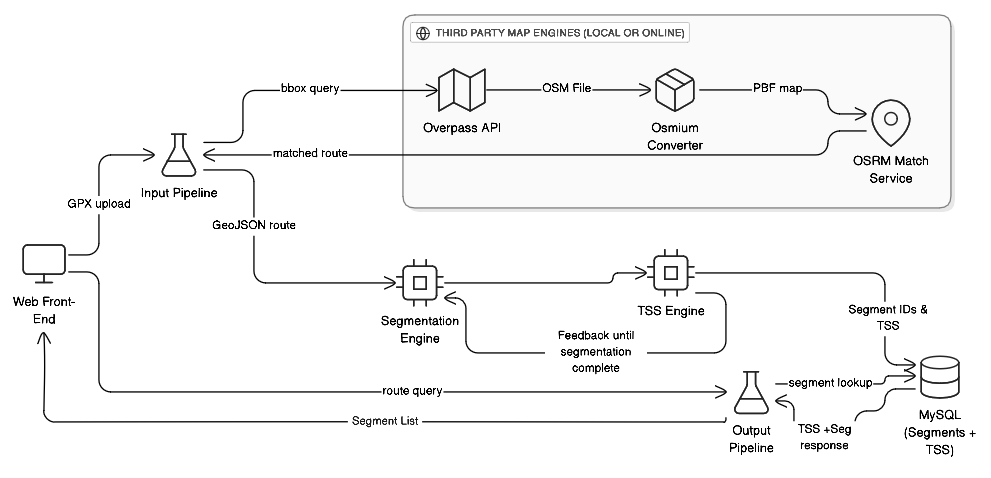
\includegraphics[width=0.9\textwidth]{archdiagram.png}
	\label{fig:archdiagram}
	\caption {High level system architecture for the Route Segmentation and Analysis System}
\end{figure}

\subsection{Architectural Views}
\subsubsection{Concept View}
The architectural concept of the system can be broken down into 3 layers:
\begin{itemize}
	\item \textbf{Presentation Layer} - This is the front end; A web application where users can either upload their GPX
	      files, or draw a route on an interactive map. This layer will communicate with the back end through HTTP API requests. This layer is mostly
	      outside the scope of the project, since I am not a front end engineer.
	\item \textbf{Processing Layer} - The beef of the project, this includes the back-end of the system, and consists of input/output pipelines,
	      and several processing engines. It will also contain several controllers, written in Python, to coordinate the pipelines and to send
	      information to and from the different engines.
	\item \textbf{Data Layer} - This layer is represented by a SQL database that stores permenant information about route segments. External APIs also
	      fall into this category, such as the Overpass API to fetch map data from online. These components provide necessary data but are mostly abstracted
	      away, in the processing layer.
\end{itemize}
\subsubsection{Functional View}
The functional view includes key modules and their responsibilities.
\begin{itemize}
	\item \textbf{Front end Web App:} Serves HTTP pages and gets information from the user.
	\item \textbf{Front End Controller:} Takes user information and routes it to correct API endpoint.
	\item \textbf{Input Pipeline Orchestrator:} Controller that handles input information routing, sending the GPX files to the pipeline, and pulling the resulting GeoJSON objects out.
	\item \textbf{Engine Orchestrator:} Takes routes, passes them to Segmentation algorithm, and handles the "two pass" system between Segmentation and TSS Engines.
	\item \textbf{DTO Orchestrator:} Formats the resulting segments, into the correct Data Object and passes it to SQL Database
	\item \textbf{Output Pipeline Orchestrator:} Receives the Route data from the Input Pipeline Orchestrator, validates it and sends it to Segmentation Engine. Gets segment list, and routes it back to front end in GeoJson format.
	\item \textbf{Segmentation Engine:} Written in C++, the engine is a specialized service that performs route segmentation and matching logic.
	\item \textbf{TSS Engine:} Takes a list of segments and the input GPX data, and assigns scores based on the training data that happens during each segment
	\item \textbf{SQL Database:} Stores all persistent segments, along with a hit count, and a list of TSS objects that have been calculated on matching segments.
	\item \textbf{Osmium Engine:} A docker service that runs a .osm to .pbf conversion and merging process. Used in the input pipeline
	\item \textbf{OSRM Matching Engine:} Another docker service that takes small GeoJson chunks, and matches them to a map network.
\end{itemize}

\subsubsection{Physical View}
Hardware deployment and network design.
%TODO: Include diagrams of network design, and list of hardware items for the project
\subsubsection{Information View}
Data Flow Diagram, and Database Schema diagrams
%TODO: Implement Data flow diagram, Relational Diagrams
\subsubsection{Behavioral View}
Use case and sequence diagrams for the system
%TODO: Create and include both use case and sequence diagrams

\subsection{Design Rationale}
The choice to go with a \textbf{Pipeline Architecture} for processing data is motivated by the main use case. Users who are looking
to find a route to ride are not interested in uploading GPX, but conversely, users who are done with their ride aren't looking to
find a route. So cyclists can be considered to be in one of two states when wishing to interact with the system, either wanting a route,
or wanting to upload their data. The two pipelines reflect this with one being a GPX upload-only pipeline, and the other one is a visualisation
pipeline that shows users what their mapped route's suitibility looks like.
A simple LAMP-like stack approach is a simple, but effective pattern that can implement this project. As of right now, this is a small scale
experiment to prove the concept. If this application becomes popular, there will be several avenues to explore for scalability, such as deploying the
system to expandable cloud services such as AWS or Azure. This is beyond the scope of the project however.

\subsection{Design Patterns and Styles}
Identify and describe any applied patterns (e.g., MVC, layered) and coding conventions.
%TODO: Research and include design patterns and coding standards

\section{Module-Level Design}
\ref{sec:moduledesign}
\subsection{Module Decomposition}
List all system modules, their interfaces, and dependencies. Include a module dependency diagram.
%TODO: Include design requirements of each python module

\subsection{Module Specifications}
For each module:
\begin{description}
	\item[Name:] Purpose and description.
	\item[Interfaces:] Inputs, outputs, and protocols.
	\item[Behavior:] Algorithmic overview or pseudocode.
	\item[Dependencies:] Internal and external module links.
\end{description}

\section{Interface Design}
\subsection{User Interface}
The user interface for the project scope will just be a basic file submission system, and an interactive mapping software that can output GeoJSON
\subsection{Software Interfaces}
The front end will send GeoJSON objects to the backend via POST. GPX files can also be sent via POST with \texttt{\small Content-Type:application/gpx+xml}
The back-end will also respond with the same GeoJSON objects back to the front-end, as well as sending segment list via POST.
REST APIs are also used to interface with third party tools such as the OSRM route matching engine, and the Overpass API.

\section{Data Design}
\subsection{Data Models}
ERD showing data entities and relationships.

\subsection{Database Schema}
Detailed table definitions, keys, indexes, and normalization rules.

\subsection{Data Dictionary}
Definitions and formats for all data elements used in the system.


\section{Standards and Compliance in Design}
List all applicable ISO/IEC, IEEE, and domain-specific standards adhered to (e.g., ISO/IEC 27001 for security).

\chapter{Implementation}
%TODO: Step-by-step go through the process of implementing the system, including issues and challenges
\label{chap:implement}
% Implementation details.

\section{Component Breakdown}
This section details the method and process of implementing each component of the system.
\subsection{Input Pipeline}
This was the first component written. It started very simple by prototyping isolating GPX files and obtaining their coordinate pairs in a list of duples.
Initially, it was written as a single file parser, but was later modified to include batch processing.
\begin{enumerate}
	\item Prototyping: Included learning about GPX file structure, and isolating data values in lists.
	\item I created a Python module that pulled data from the Overpass API, and tested it by putting in some bounding box (bbox) coordinates.
	\item I then set up the Python virtual environment, which would gather the required modules from \texttt{requirements.txt}.
	\item The next logical step was to take the GPX file, and parse it for the coordinates, then extract the min and max latitude and longitudes. I then created
	      a function that generated a bbox from the GPX file, and used that to get OSM data.
	\item I researched OpenSourceRoutingMachine (OSRM), which was a framework that had several useful functions, one of which was match GPS points to
	      an OSM network. Unfortunately, the files downloaded from Overpass were only of the .osm file type, which is essentially just XML. I needed
	      to convert it to Protocolbuffer Binary Format (.pbf) for OSRM to be able to use it.
	\item I did more research, and found that Osmium provided the tools necessary to convert to .pbf, as well as other tools such as map merging (which would prove useful later
	      for batch processing). However, since I wanted to keep all the necessary environments enclosed within the pipeline directory, I couldn't use osmium directly in Python,
	      since there was no proper module for it, but I decided instead to set up my own Osmium engine, by creating a docker image from Ubuntu, and using a Dockerfile to install and set up
	      Osmium on the container. I then wrote a Docker Compose file that would set up the necessary volumes in the pipeline directory, and set the entrypoint to "osmium". I also wrote a few scripts
	      that would merge and then convert every .osm file in the input directory.
	\item The \texttt{run\_pipeline.sh} bash script was the main file that orchestrated all of the input directions, such as creating and removing directories, and running
	      Docker. I created the script around this point, after the osmium docker compose, so I could start automating the process as we went along.
	\item After Osmium, I had successfully created a script that took GPX files and generated a map from them in .pbf format. At this point it was prudent of me to start
	      actually doing formal testing, so I created a few test functions that would run in the background and collect variable information for me to see. I also created
	      a test script that would convert the .pbf file into a viewable map, with the .gpx coordinates overlaid. \ref{fig:pbfmap} shows this map:
	      \begin{figure}
		      \centering
		      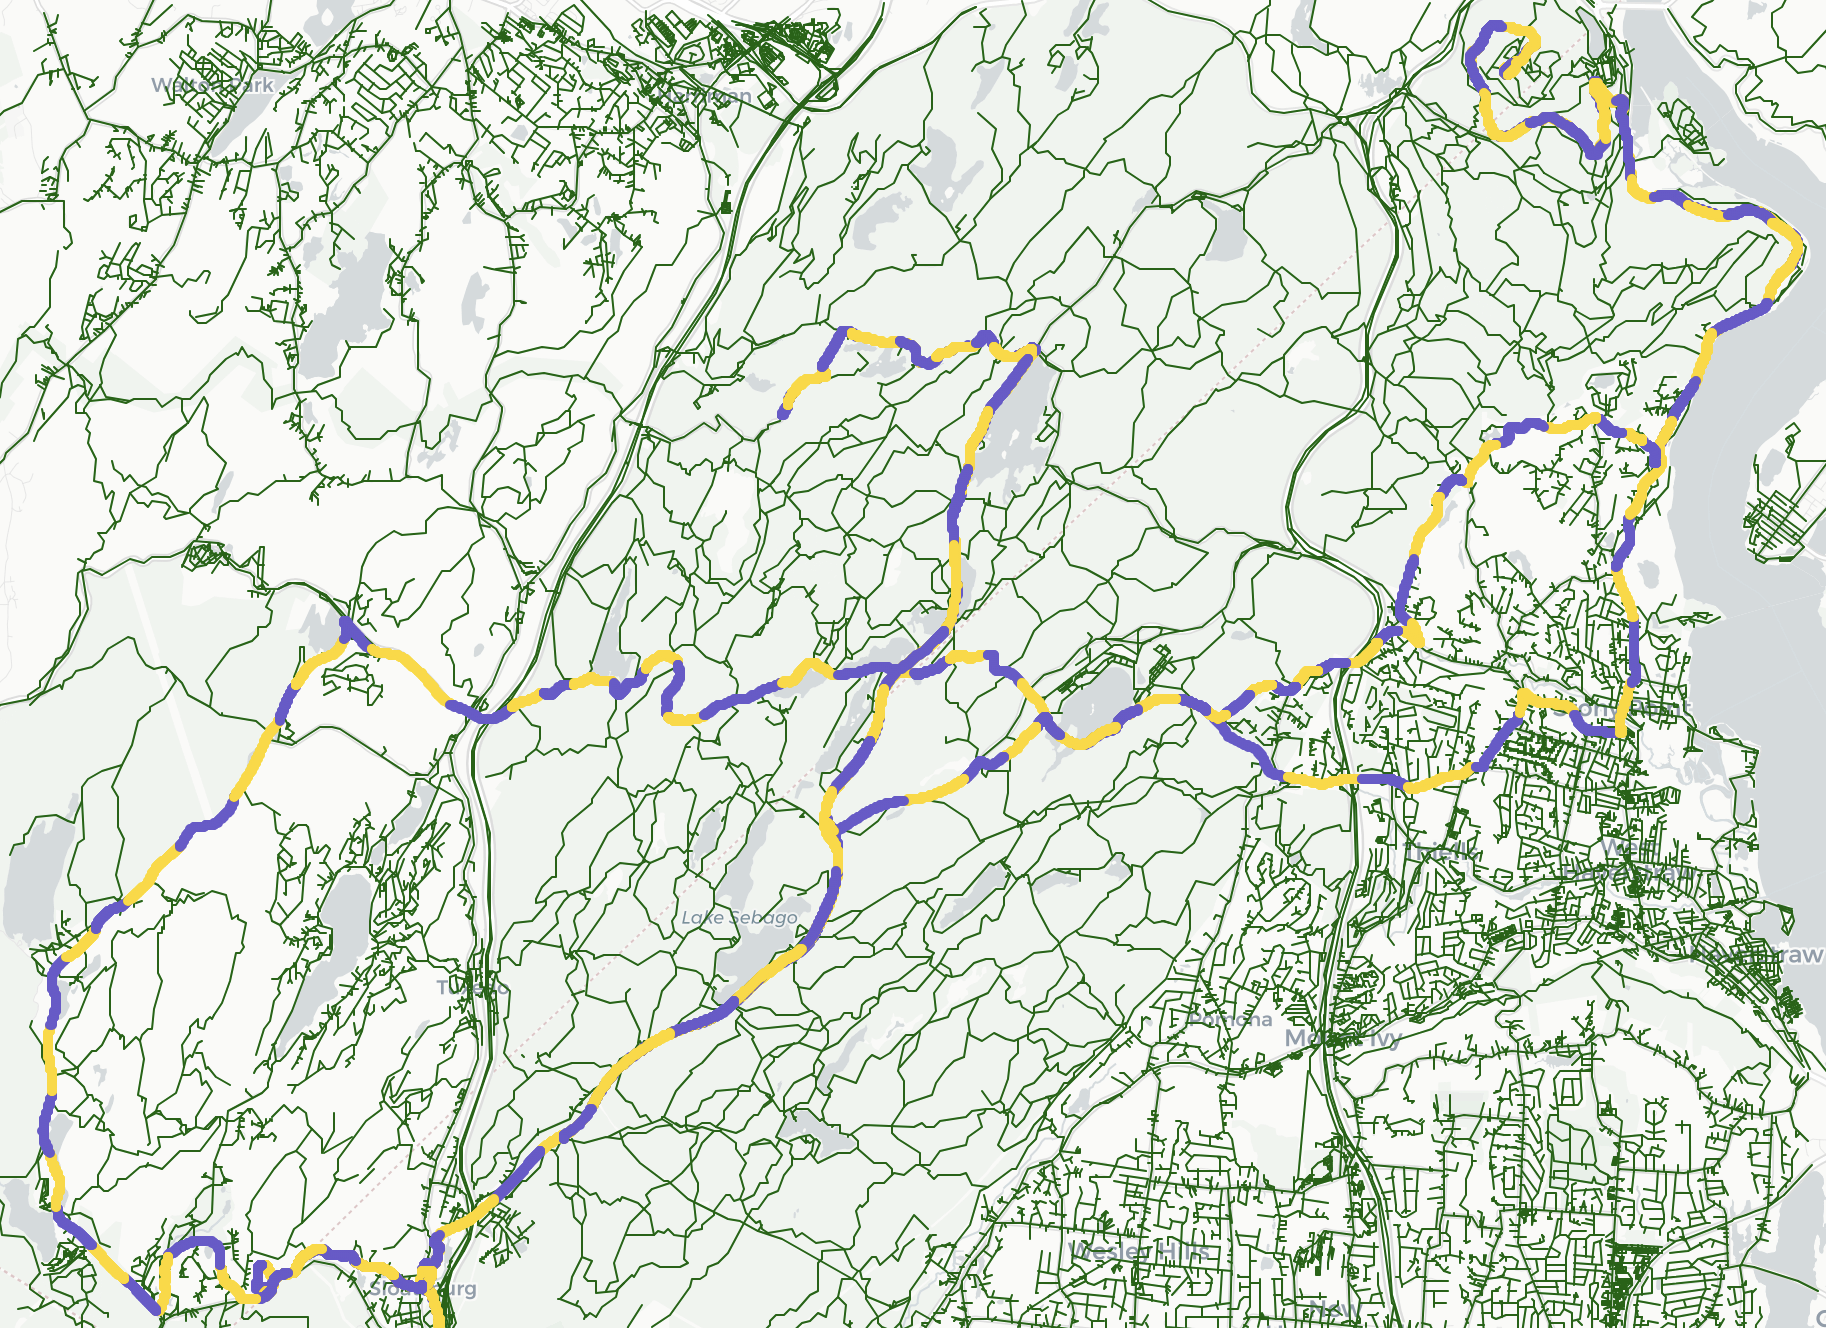
\includegraphics[width=0.8\textwidth]{pbf_map.png}
		      \label{fig:pbfmap}
		      \caption{A visual representation of the Road network used for testing the pipeline. Green roads are the downloaded .pbf map edges, and the blue and yellow
			      line is the series of GPX points plotted over the top to verify that the bounds had successfuly covered the route}
	      \end{figure}
	\item Now I started creating another Docker instance for OSRM. There exists a docker container image "osrm-backend", which I ran in detached mode, and assigned input and output volumes.
	      In the backend, there are a few functions that were necessary to call before I started the match service. I first had to download a profile.lua file from OSRM's website. This
	      contained all the settings and optimisations that I could change to adjust the matching algorithm. This worked by giving certain road types different speed limits. I adjusted them to roughly what
	      I felt I could do on those types of roads on a bike. For example, on a road, I put 35 (units are Km/hr), on gravel I put 25, and I put even less on other types of roads that I felt were unattractive
	      to cycle on. I set the weight parameter to "duration", which essentially made it so the speed value became a weighting unit. The higher the number, the more likely the match engine would choose to go
	      on that route. When testing, I ran into an issue where no matter what, I couldn't get the route to go the right way, but it turned out I actually didn't have the right road defined. The road turned out
	      to be a "trunk" highway, when that type didn't exist by default in the profile.lua. This showed me that the file isn't perfect, and will require tweaking over time. However, after a few days of tweaking,
	      I came up with a profile that seemed pretty good and could match 95\% of my test routes with 99\% or more accuracy. I feel this is highly individual, but in the future, it could be fun to try to automate
	      the profile.lua values to hyper-optimise the matching algorithm.
	\item After running the profile.lua through the OSRM engine, I then created another Python module called \texttt{batch\_route\_calc.py}. This file, as named, was the first attempt
	      at batch processing files. However, this wasn't at the time because I needed to parse multiple GPX files. It actually came about because at this point I realized that matching an entire GPX file
	      in one go is a bad idea. Some of my test files had over 10,000 GPX points, and needless to say, sending all 10,000 through a REST API is difficult at the best of times, but because OSRM is slightly outdated,
	      the only way to process the map data is through GET requests to the /match endpoint, with the data in the URL itself. Sending 10,000 coordinates, each with between 15 and 20 characters would be impossible, so I had to come up with a solution.
	\item My solution was two-fold. Firstly, I would break the GPX file into chunks. I went back to my first python script, and added a function that would take the gpx files, format into .json files of a smaller length, and batch process them with OSRM.
	      I was successful in creating the "chunks" as I called them. But the issue I ran into was the fact that I had to still make over 100 GET requests, since the largest reasonable amount of data I could send in 1 go was 100 GPS coordinates.
	\item I solved this problem by parallelizing the script. I used ThreadPoolExecutor to run multithreaded batch processing on the GPX file. This sped things up significantly, and allowed me to process the GPX file in seconds rather than closer to a minute.
	\item I started also parallelizing other processes, such as the API calls to Overpass, and the input/output file operations. These are the tasks that benefit the most from multithreading.
	      %TODO: Talk about the dynamic radius function, as well as any other functions that were not talked about
	\item Next I had to merge the many route chunks that were generated from OSRM. I was able to optimise this to O(log n) with tree recursion, as well as multithreading within each tree level. To do this, I essentially
	      just performed merge on every pair, and recursively called the merge function until the base case where there was only 1 value, in which case we were finished. This worked well, although I had a few instances
	      where the recursion broke because the merge function wasn't working correctly, and I got infinite recursion, which is always fun.
	\item After merging, I visualised the connected route with Folium, and compared the route to the GPX file. I overlaid both on the same map to check for issues. This is also where I started manipulating the profile.lua file in OSRM directory
	      to try and get matching as accurate as I could. After a few days I got it to the previously stated accuracy of roughly 99\% for most of my files. The 5\% of files that I could not get that accurate ended up being outliers anyway. Most of them
	      either had large amounts of GPS noise, or were not on mapped roads, or were going throught junctions or along bike paths that ran with the road I was on. All of these are not huge considerations however,
	      as the main goal of the system isn't to accurately map routes, but to quantify training suitibility. If there is a bike path nearby, then most of the time, that will end up being
	      a little bit more suitible than the road, and if not, they're close enough together that anyone out on the road can choose which one they prefer.
	\item As well as manipulating the profile settings, I also played around with the radius distance. The radius is a parameter fed to OSRM as an array. 1 value per GPS coordinate, and it's meaning
	      is the distance away from the coordinate to search for a matching route. If the value is too small, GPS noise could push the coordinate away too far from the road. If radius is too large, then
	      the algorithm may start considering routes that were higher weighting, but strayed too far from the real route.
	\item The very last step in the pipeline is to enrich the route map with OSM metadata, such as road names, road width, road type, speed limit, etc. This was done with a python script called \texttt{enrich.py}.
	      The module took the waypoints in the GeoJSON file, and mapped them onto OSM ways using OSMnx's nearest node function. Each node was assigned a "way", and a file was created that stores that way, along with the array of waypoints, in the order they occured.
	      This basically provides a mapping of GPS coordinates to OSM ways, and also provides the lowest level of granularity for our segmentation algorithm to work with.
\end{enumerate}
\subsubsection{Data Stream}
The data going in was the GPX file, and the settings.yml that controlled parameters such as chunk size (of the gps chunks), and dynamic radius window, which determined how wide of a window to check for variance to adjust the match search radius.
% ...

\subsection{Segmentation Engine}

\subsection{TSS Engine}
% ...

% Add more as needed
\section{Testing and Results}
% Testing procedures and results.

\chapter{Results and Conclusions}
\label{chap:results}
% Final results and conclusions.

\chapter{Further Discussions and Research Gaps}
\label{chap:discussion}
% Discussion and gaps.

\appendix
\chapter{Appendix}
\label{chap:appendix}
\section{Further Reading}
% References for further reading.

\section{Source Code}
% Include code listings or reference external files.

\section{File Structure}
% Describe directory/file organization.

\section{Additional Documentation}
% Any extra docs.

%---------------------------------------------------------------------------
% Bibliography
%---------------------------------------------------------------------------
\bibliographystyle{unsrtnat}
\bibliography{references}

\end{document}

